\documentclass[12pt,final]{report}

\usepackage{style}
\usepackage{dhbwTitlepage}
\usepackage{xcolor}
\usepackage{color}
\usepackage{svg}
\usepackage{seqsplit}
\usepackage{rotating}
\usepackage{listingsutf8}
\usepackage{fancyhdr}
\usepackage{appendix}
\usepackage{censor}
\usepackage{tipa}

\definecolor{dkgreen}{rgb}{0,0.6,0}
\definecolor{gray}{rgb}{0.5,0.5,0.5}
\definecolor{mauve}{rgb}{0.03,0.6,0.18}
\definecolor{lgray}{rgb}{0.2,0.2,0.2}
\definecolor{lorange}{rgb}{1,0.7,0.37}
\definecolor{purple}{rgb}{0.8,0.4,1}

\lstset{frame=tb,
  language=C++,
  aboveskip=7mm,
  belowskip=3mm,
  showstringspaces=false,
  columns=flexible,
  basicstyle=\linespread{0.9}\small\ttfamily,
  numbers=none,
  numberstyle=\tiny\color{gray},
  identifierstyle=\color{lgray},
  keywordstyle=\color{blue},
  commentstyle=\color{dkgreen},
  stringstyle=\color{mauve},
  breaklines=true,
  breakatwhitespace=true,
  tabsize=3,
}

% Rechtschreibprüfung
% Kommandozeile für die Rechtschreibprüfung dafür: lualatex '\def\spelling{}\input{Arbeit}'
\ifdef{\spelling}{
    \usepackage{spelling}
    \usepackage{microtype}
    \DisableLigatures{encoding = *, family = *}
}

% Zensieren
% Kommandozeile für eine unzensierte Version: lualatex '\def\uncensored{}\input{Arbeit}'
\ifdef{\uncensored}{
    \StopCensoring
}

\def\censorruleheight{0.1ex}
\def\censorruledepth{0.5ex}


% "Metadaten"
\title{Evaluierung von Tools zum Auffinden von Undefined Behavior}
\project{T3000}
\author{Christoph Böhringer}
\supervisor{Dipl.-Inform. (FH) Thomas Weller}
\studentNumber{3275565}
\class{TINF18IN}
\company{Mitutoyo CTL Germany GmbH}
\date{21.06.2021}

% Initialisierungen für Abkürzungsverzeichnis
\loadglsentries{Acronyms.tex}
\makeglossaries
\setglossarystyle{altlist}
\addbibresource{literature.bib}

% Formatierung der Kopfzeile
\fancyhf{}                              % Standarddefinitionen der Kopfzeile löschen
\fancyfoot[C]{\thepage}                 % Seitenzahl in der Mitte der Fußzeile angeben
\renewcommand{\headrulewidth}{0pt}
\renewcommand{\footrulewidth}{0.4pt}
\fancypagestyle{plain}{
    \fancyfoot[C]{\thepage}
    \renewcommand{\footrulewidth}{0.4pt}
}

\begin{document}
    \pagenumbering{Roman}
    \maketitle                                  % Titelblatt
    % \chapter*{Sperrvermerk}

Der Inhalt dieser Arbeit darf weder als Ganzes noch in Auszügen Personen außerhalb des Prüfungsprozesses und des Evaluationsverfahrens zugänglich gemacht werden, 
sofern keine anderslautende Genehmigung der Ausbildungsstätte vorliegt.                 % Sperrvermerk
    \chapter*{Erklärung}
\label{ch:erklaerung}

Ich versichere hiermit, dass ich meine 
\makeatletter
\@project
\makeatother
\ mit dem Thema 
\makeatletter
\glqq{}\@title\grqq{}
\makeatother
\ selbstständig verfasst und keine anderen als die angegebenen Quellen und Hilfsmittel benutzt habe.

Ich versichere zudem, dass die eingereichte elektronische Fassung mit der gedruckten Fassung übereinstimmt.

Falls gleichwertige Entscheidungen getroffen werden mussten, wurden diese von mir
entschieden, außer es ist anders angegeben.

\vspace{2.0cm}
\underline{\hspace{12cm}}\\
Ort \hspace{3cm} Datum \hspace{2cm} 
\makeatletter
\@author
\makeatother         % Erklärung
    \chapter*{Abstract}
\label{ch:abstract}
\addcontentsline{toc}{chapter}{\nameref{ch:abstract}}
In einem Softwareprodukt trat bei der Umstellung von 32 Bit auf 64 Bit ein Fehler auf,
dessen Ursache sich vermutlich auf Undefined Behavior von C++ zurückführen lässt. Diese Arbeit soll den Nachweis erbringen oder widerlegen,
dass Undefined Behavior die Ursache für den Fehler war. Optional kann eine mögliche Erklärung gesucht werden,
warum der betroffene Code in der 32 Bit Version keinen Fehler verursacht hat.

Das betroffene Projekt wurde vor der Umstellung mehrere Jahre lang nicht verändert. Es muss daher davon ausgegangen werden,
dass sich ähnliche Fehler damals auch an anderen Stellen eingeschlichen haben, jedoch noch nicht  bemerkt wurden.
Die Arbeit soll untersuchen, ob weitere Fehler vom Typ Undefined Behavior in diesem Projekt vorliegen.

Um Fehler dieser Art auch in anderen Projekten auszuschließen, sollen Tools gesucht und evaluiert werden,
mit denen die Fehler automatisiert gefunden und berichtet werden können. Falls kein passendes Tool existiert, soll aufgezeigt werden,
mit welchem manuellen Vorgehen solche Stellen erkannt werden können.

Die Tools sollen möglichst mit den bestehenden Entwicklungsumgebungen verwendet werden können und idealerweise alle Arten von
Undefined Behavior erkennen.

Hinweis: Da in der Arbeit Source Code der Mitutoyo CTL Germany GmbH offengelegt wird, ist die Arbeit unter Verschluss zu halten.
             % Abstract
    \tableofcontents                            % Inhaltsverzeichnis
    \listoffigures                              % Abbildungsverzeichnis
    \listoftables                               % Tabellenverzeichnis
    \printglossary[
      type=\acronymtype,
      title={Abkürzungen},
      nogroupskip]           % Akronyme
    \printglossary[type=main]                         % Glossar
    %\printacronyms
    %\printglossary[
    %  type=\acronymtype,
    %  title={Abkürzungen},
    %  nogroupskip
    %]                                           % Abkürzungsverzeichnis
    %\printglossary[type=main]                   % Abkürzungsverzeichnis
    \clearpage
    \pagenumbering{arabic}
    \pagestyle{fancy}
    \chapter{Einleitung}
\label{ch:Einleitung}

In einem Softwareprodukt trat bei der Umstellung von 32 Bit auf 64 Bit ein Fehler auf,
dessen Ursache sich vermutlich auf Undefined Behavior von C++ zurückführen lässt. Diese Arbeit soll den Nachweis erbringen oder widerlegen,
dass Undefined Behavior die Ursache für den Fehler war. Optional kann eine mögliche Erklärung gesucht werden,
warum der betroffene Code in der 32 Bit Version keinen Fehler verursacht hat.

Das betroffene Projekt wurde vor der Umstellung mehrere Jahre lang nicht verändert. Es muss daher davon ausgegangen werden,
dass sich ähnliche Fehler damals auch an anderen Stellen eingeschlichen haben, jedoch noch nicht  bemerkt wurden.

Um Fehler dieser Art auch in anderen Projekten auszuschließen, sollen Tools gesucht und evaluiert werden,
mit denen die Fehler automatisiert gefunden und berichtet werden können. Falls kein passendes Tool existiert, soll aufgezeigt werden,
mit welchem manuellen Vorgehen solche Stellen erkannt werden können.

Die Tools sollen möglichst mit den bestehenden Entwicklungsumgebungen verwendet werden können und idealerweise alle Arten von
Undefined Behavior erkennen.
             % Einleitung
    \chapter{Requirements Engineering}
\label{ch:requirements}

Das Requirements Engineering bezieht sich in diesem Projekt auf das Erfassen von Stakeholdern und das Ermitteln von Anforderungen.

Wegen fehlenden oder falschen Anforderungen können viele Projekte nicht die gewünschten Ziele
erreichen \cite[S.~4-9]{Ebert:SystematischesReqEng}. Aus diesem Grund ist es sinnvoll zum Beginn eines Projektes Stakeholder zu erfassen,
eine Vision aufzustellen und Anforderungen an des Endprodukt zu ermitteln.


\section{Stakeholder}
\label{sec:stakeholder}

Die Stakeholder-Analyse identifiziert wichtige Anspruchsträger des Projektes.
Die nachfolge Tabelle wurde nach \cite[S.~58-60]{Ebert:SystematischesReqEng} ausgefüllt.
Eine Analyse der Verantwortung einzelner Stakeholder entfällt, da sich diese in dieser Arbeit mit der Rolle deckt. Zusätzlich arbeit jeder
Stakeholder in der gleichen Firma/Abteilung, weshalb die Spalte \glqq{}Verfügbarkeit\grqq{} ausgelassen wird.

\begin{table}[H]
    {
        \tiny
        \begin{tabularx}{\linewidth}{|X|X|X|X|X|}
            \hline
            Rolle
             & Name
             & Aufgabenbeschreibung
             & Hintergrundinformationen
             & Konfliktpotenzial
            \\
            \hline
            \cline{1-5}
            Gutachter Intern
             & TW
             & Aus- und Weiterbildung des Personals
             & Betreut/bewertet die Studienarbeit \newline
            Beratung/Analyse von \ref{sec:windbg}
             &
            \\
            \cline{1-5}
            Gutachter DHBW
             &
             & Gutachter
             & Bewertet die Studienarbeit
             &
            \\
            \cline{1-5}
            Entwickler
             &
             & Softwareentwicklung
             & Soll Tools benutzen um \gls{ub} zu vermeiden
             &
            \\
            \cline{1-5}
            Tester
             &
             & Testen der Software
             & Weniger Fehler in der Software erleichtern die Arbeit
             &
            \\
            \cline{1-5}
            Architekt
             & DB
             & Kontrollieren des Source Code falls Selbstkontrolle nicht klappt
             & Hat den Bug bearbeitet und behoben
             &
            \\
            \cline{1-5}
            Build Manager
             & TF
             & DevOps
             & Verantwortlich für TFS Zugang und Build Prozesse
             &
            \\
            \cline{1-5}
            Geschäftsführer
             & PK
             & Ressourcenverteilung (Zeit, Verfügbarkeit der Trainer, \dots)
             & Finanziert Studium \newline
            Finanziert Tool
             &
            \\
            \hline
        \end{tabularx}
    }
    \caption{Stakeholder}
    \label{tab:stakeholder}
\end{table}
    \chapter{Undefined Behavior}
\label{ch:ub}

\section{Was ist Undefined Behavior?}
\label{sec:ub_was}

Der C++ Standard definiert \gls{ub} wie folgt: \newline
\glqq{}Permissible undefined behavior ranges from ignoring the situation completely with unpredictable results, to behaving during translation or program execution in a
documented manner characteristic of the environment [...]\grqq{}.\cite[S.8]{book:cpp-standard} \newline
Das Auftreten von \gls{ub} führt also entweder zu zufälligem Verhalten des Codes oder zu einem umgebungsspezifischem Verhalten.

Eben dieses zufällige Verhalten führte zu dem in \ref{sec:windbg} analysierten Bug. Ein Problem an zufälligem Verhalten ist, dass das Verhalten nicht zwingend zu einem
Absturz des Programms führt, sondern nur einen zufälligen Wert liefert. Dieser Wert kann nun Messergebnisse verfälschen und somit darauf schließen lassen, dass die gesamte
Software fehlerhaft ist.

\section{Ursachen von Undefined Behavior}
\label{sec:ub_ursachen}

Der C++ Standard\cite{book:cpp-standard} beschreibt über 500 verschieden Ursachen für \gls{ub}. Eine genauere Beschreibung aller Ursachen wird aufgrund der Anzahl nicht durchgeführt.

\textbf{Undefinierte Variablen:} Entgegen erster Annahmen, dass undefinierte Variablen zwingend zu \gls{ub} führen, ist dies seit 2014 nicht mehr der Fall, da sich die
\glspl{callingconvention} geändert haben. Der Wert einer undefinierten Variable ist nun als \glqq{}indeterminate\grqq{} festgelegt\cite[S.63]{book:cpp-standard}.
\gls{ub} tritt erst dann auf, wenn die undefinierte Variable ausgewertet wird (vgl. \ref{subsec:indeterminate}). Hierzu bestehen allerdings Ausnahmen, wenn \verb|unsigned|
Variablen verwendet werden. \cite[S.63]{book:cpp-standard}

\textbf{Nullpointer Dereferenzierung:} Der Versuch den Wert der Adresse eines Nullpointers zu lesen, endet in \gls{ub}. \cite[S.188]{book:cpp-standard} (vgl. \ref{subsec:nullpointer})

Einige weitere Ursachen von \gls{ub} sind:
\begin{itemize}
    \item Signed overflow \cite[S.74]{book:cpp-standard}
    \item Modifizieren eines \verb|const| Objekts \cite[S.174]{book:cpp-standard}
    \item Data races \cite[S.1376]{book:cpp-standard}
    \item Invalid pointer value \cite[S.67]{book:cpp-standard}
    \item Zugriff außerhalb der Lebensdauer \cite[S.35]{book:cpp-standard} (vgl. \ref{subsec:outside-lifetime})
\end{itemize}

\section{Warum wird Undefined Behavior benutzt?}
\label{sec:ub_warum}

\gls{ub} ermöglicht dem \gls{compiler} Code-Optimierungen durchzuführen, indem der \gls{compiler} davon ausgeht, dass das Programm nur definierte Operationen durchführt. \cite[S.633]{book:taming-ub}

Das Verwenden von \gls{ub} resultiert in einer Optimierung der Perfomance. Für diese wird jedoch die Vorhersehbarkeit und Sicherheit des Codes eingeschränkt. \cite[S.633]{book:taming-ub} \\
Es wird den Entwicklern überlassen das Auftreten von \gls{ub} zu verhindern oder zu minimieren.

Andere Programmiersprachen, wie Java, sollen in ihrer \gls{ir} das Auftreten von \gls{ub} verringern oder verhindern. \cite[S.633]{book:taming-ub}
    \chapter{Toolfindung}
\label{ch:toolfindung}

In diesem Kapitel werden vier Tools untersucht, welche \gls{ub} auffinden sollen:
\begin{itemize}
  \item PC-lint Plus \cite{misc:pclintplus}
  \item Cppcheck \cite{misc:cppcheck}
  \item \gls{ubsan} (wird von GCC und Clang++ verwendet) \cite{misc:ubsan}
  \item PVS-Studio \cite{misc:pvsstudio}
\end{itemize}
Die Tools werden dabei anhand einer Bewertungsmatrix mit den Anforderungen F-1 bis F-6, NF-2 und NF-3 bewertet. Die Anforderungen sind mit Zahlen von eins bis fünf gewichtet, wobei
eine höhere Zahl für eine höhere Relevanz steht. Bei F-1 und F-2 wird das Erfüllen der Anforderung in Form einer Warnung mit 70\% gewertet. 100\% werden vergeben, wenn das Tool einen
Error ausgibt.
\begin{figure}[htpb]
  \centering
  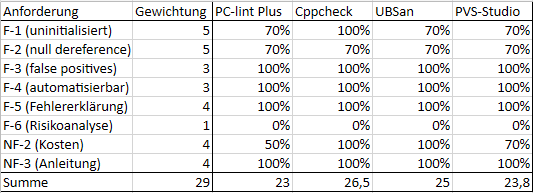
\includegraphics[width=0.8\textwidth]{toolfindung}
  \caption{Bewertungsmatrix}
  \label{img:toolfindung}
\end{figure}

Die Erfüllung der Anforderungen F-1 und F-2 wird in \ref{sec:codeanalyse} beschrieben. \newline
Da jedes Tool von der Kommandozeile aus bedienbar ist, sind alle Tools automatisierbar. Dies ermöglicht auch eine Integration in Projekte jeder Art. Für PVS-Studio existiert jedoch
zusätzlich eine Extension für Visual Studio \cite{misc:pvsplugin}. \newline
Eine Risikoanalyse wird von keinem Tool zur Verfügung gestellt. \newline
Im Gegensatz dazu verfügt jedes Tool über eine Dokumentation. Beim Aufruf am 02.02.2021 referenzierte die Dokumentation von PVS-Studio (\cite{misc:pvsdoku}) nicht mehr vorhandene Seiten. Zusätzlich
funktionierte die integrierte Suchfunktion nicht mit einzelnen Wörtern. Dies ist aktuell (letzter Aufruf 16.06.2021) nicht mehr der Fall.\newline
Sowohl Cppcheck als auch \gls{ubsan} sind kostenfrei verfügbar. \newline
PVS-Studio kostet im ersten Jahr, für ein Entwicklerteam mit 10-30 Entwicklern, 21.000€. Für jedes folgende Jahr belaufen sich die Kosten auf 80\% des Preises (16.800€).\newline
Die zuständigen Stelle von PC-Lint Plus hat bezüglich auf eine Preisanfrage, zum aktuellen Zeitpunkt, noch keine Rückmeldung gegeben. Aus diesem Grund wird NF-2 bei diesem Tool
vorläufig mit 50\% bewertet.

\section{Codeanalyse}
\label{sec:codeanalyse}

\subsection{PVS-Studio}

\begin{figure}[htpb]
  \centering
  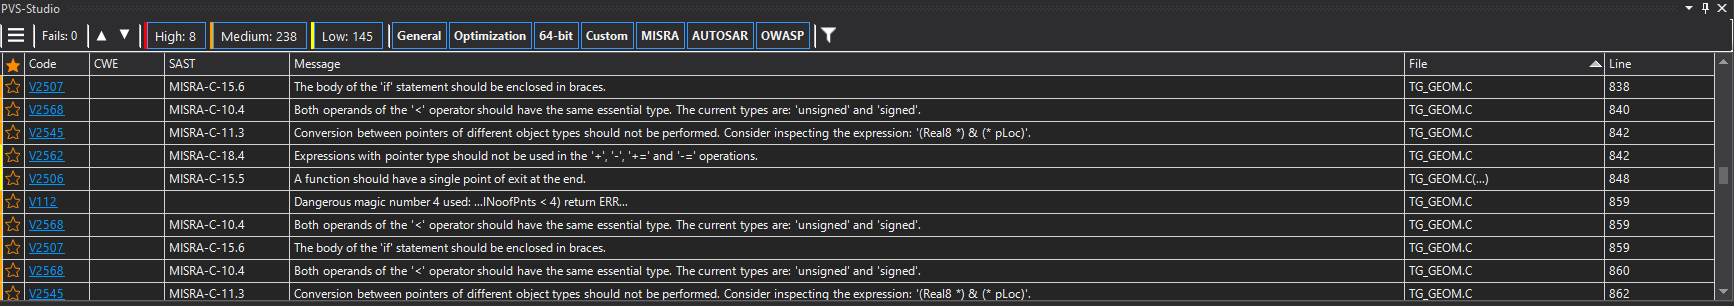
\includegraphics[width=1\textwidth]{pvs-tg-geom}
  \caption{Ausschnitt der von PVS-Studio gemeldeten Fehler}
  \label{img:pvs-tg-geom}
\end{figure}

Die Extension von PVS-Studio für Visual Studio kann circa 600 verschiedene Fehler erkennen und mit einer kurzen Beschreibung ausgeben. Es kann dabei frei ausgewählt werden, welche Arten von
Fehlern gemeldet werden sollen. \newline
Wird nur die Datei \glqq{}TG\_GEOM.C\grqq{} analysiert, so gibt das Tool insgesamt 361 Fehlermeldungen in der Datei aus. Die Fehler werden dabei in die Kategorien \glqq{}High\grqq{}
(0 Fehler), \glqq{}Medium\grqq{} (227 Fehler) und \glqq{}Low\grqq{} (134 Fehler) eingestuft. Zusätzlich in \ref{img:pvs-tg-geom} gemeldete Fehler stammen aus anderen Dateien.

PVS-Studio erkennt keine uninitialisierten Variablen in der analysierten Datei, obwohl dies beispeilsweise in Zeile 992 der Fall ist. Eine erste Annahme, dass dies geschieht, weil die
Variablen nicht direkt ausgewertet werden, sondern über verschiedene Dateien in verschiedenen Funktionen aufgerufen werden, wurde wiederlegt. Auch eine Analyse der gesamten Solution
ergab keinen Fehler, welcher sich mit uninitialisierten variablen beschäftigt. \newline
Im Kontrast dazu erkennt PVS-Studio alle erwarteten Fehler im Code-Beispiel \ref{subsec:indeterminate}. Durch eine Integration, und erfolgreiche Fehlererkennung, des Beispiel-Codes in
\glqq{}TG\_GEOM.C\grqq{} wurde widerlegt, dass PVS-Studio mit der Menge an Code überfordert ist. \newline
PVS-Studio erkennt nicht initialisierte Variablen erfolgreich in dem Code-Beispiel. In \glqq{}TG\_GEOM.C\grqq{} werden allerdings keine uninitialisierten Variablen gefunden. Dafür
werden zahlreiche andere Fehler markiert. PVS-Studio erhält somit für F-1 eine Bewertung von 65\%. 50\% für eine korrekte Fehlererkennung im Beispielcode und 15\% für eine allgemein
sehr gute Fehlererkennung.

PVS-Studio markiert den in \ref{subsec:nullpointer} beschriebenen Code erfolgreich als fehlerhaft und erkennt fehlerhafte Benutzung von Pointern beispielsweise in
\glqq{}CryptoPP/algparam.h\grqq{} Zeile 36. Somit bekommt das Tool eine Wertung von 80\% für F-2. 20\% werden abgezogen, da keine explizite Nullpointerdereferenzierung
aufgezeigt wurde.

Anmerkung: Die Analysezeit für die gesamte Solution betrug circa eine Minute. \newline
Alle weiteren Tools werden unter den gleichen Bedienungen, wie PVS-Studio getestet.

\subsection{Cppcheck}

\begin{figure}[htpb]
  \centering
  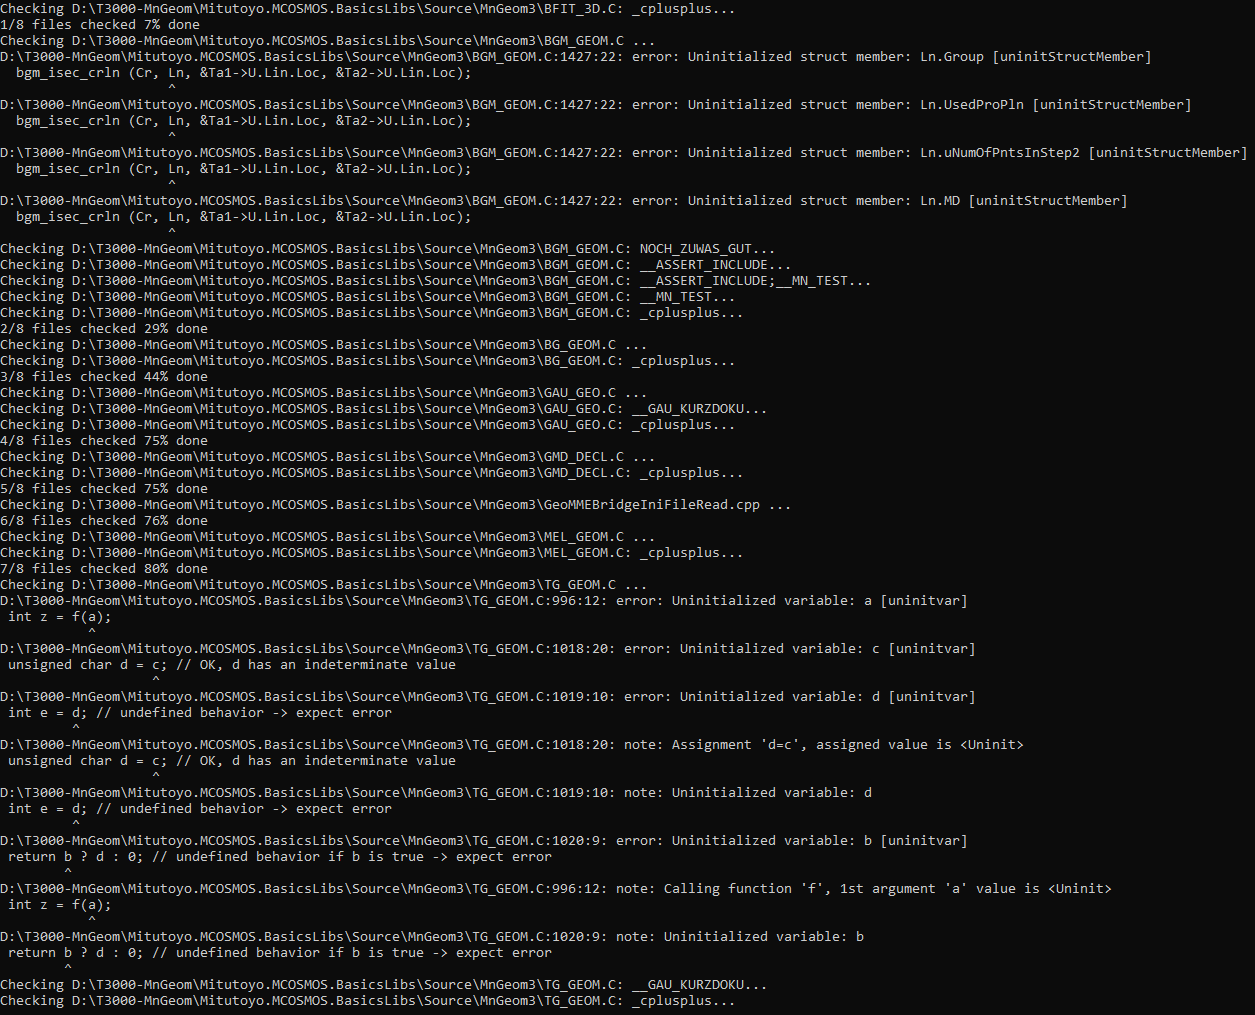
\includegraphics[width=1\textwidth]{cppcheck-mngeom}
  \caption{Von Cppcheck im Ordner MnGeom3 erkannte Fehler}
  \label{img:cppcheck-mngeom}
\end{figure}

Im Ordner \glqq{}MnGeom3\grqq{} erkennt Cppcheck die in \glqq{}TG\_GEOM.C\grqq{} vorhandenen Test-Fehler und zusätzlich uninitialisierte Variablen in \glqq{}BGM\_GEOM.C\grqq{}. Letztere
sind zu Beginn nicht initialisiert, zum Zeitpunkt, an welchem Cppcheck diese als Fehler markiert, sind die Variablen allerdings initialisiert. \newline

Cppcheck erkennt Nullpointerderefernzierung im Code-Beispiel \ref{subsec:nullpointer}, auch in der Solution von MBasicLibs werden beispielsweise in \glqq{}CryptoPP/algparam.h\grqq{}
mehrere Nullpointerdereferenzierungen markiert.

Für F-1 erhält Cppcheck 45\%. 50\% für eine korrekte Fehlererkennung im Beispielcode und -5\% für false positives. \newline
Für F-2 erhält Cppcheck 75\%. 50\% für eine korrekte Fehlererkennung im Beispielcode und 25\% für das Erkennen von Nullpointerderefernzierungn in MBasicLibs. Dort wurden allerdings
jedes Auftreten des Schlüsselworts \textit{NULL} als Nullpointerdereferenzierung markiert. Deshalb keine 100\%.

\section{Auswahl}
\label{sec:auswahl}

Cppcheck erreicht in der Bewertungsmatrix (Abbildung: \ref{img:toolfindung}) die höchste Punktzahl und ist somit Sieger der Bewertung und daraus resultierend die Toolempfehlung.
Jedoch zeigen die anderen Tools keine übermäßigen Abweichungen auf und können auch in Betracht gezogen werden, falls beispielsweise eine Integration in Visual Studio gewünscht ist
(PVS-Studio). \newline
Zur optimalen Toolfindung empfiehlt sich somit das Testen der einzelnen Tools in einem größeren Projektumfeld. Die kostenpflichtigen Tools bieten für diesen Zweck kostenlose
Testlizenzen an. Attraktiv ist hierbei PVS-Studio, da dieses mit einer Extension in Visual Studio integriert werden kann. Allerdings ist PVS-Studio allgemein weniger bekannt und die Suche nach Online-Hilfe ist somit schwieriger. \newline
Zusätzlich können die kostenfreien Tools ergänzend zu dem schlussendlich ausgewählten Tool eingesetzt werden. Dies ermöglicht eine höhere Fehlerabdeckung, garantiert allerdings nicht,
dass neue, beziehungsweise mehr, Fehler erkannt werden. Da das Einsetzen der kostenlosen Tools nur Zeit kostet, ist der Einsatz dieser immer eine Überlegung wert.
    \chapter{Zusammenfassung}
\label{ch:zusammenfassung}

Mit dieser Arbeit sollte ein kontextabhähniger Kommunikationsassistent entwickelt werden (\ref{sec:vision}). Dies wurde in Form einer Applikation namens Strike Up umgesetzt.

Strike Up ist eine für Android entwickelte App, welche dem/der Nutzer/-in ermöglicht ein eigenes Profil, sowie Profile von Gesprächspartnern/-innen, zu erstellen. Diese Profile enthalten bevorzugte und gemiedene Tags, anhand welcher während einer Konversation Fragen ausgewählt und vorgeschlagen werden. Des Weiteren haben automatisch generierte und durch den/die Nutzer/-in ausgewählte Umgebungsvariablen einen Einfluss auf die Auswahl der Fragen. \newline
Fragen beziehen sich somit auf bevorzugte und weniger bevorzugte Themen des/der Nutzers/-in und des Gegenübers, sowie auf die Umgebung der Konversation.

Um Strike Up nutzern zu können, müssen sich Nutzer/-innen mit einer E-Mail-Adresse und einem Passwort anmelden. Anschließend wird eine Altersbestätigung, sowie eine Einwilligung zur Speicherung der Daten gefordert.

Jegliche von Strike Up zur Verfügung gestellte, sowie durch den/die Nutzer/-in erstellte, Daten werden in der, von Google gehosteten, Cloud-Datenbank Firebase gespeichert. Nutzer/-innen können dabei alle Teile der Datenbank lesen, welche keine Informationen anderer Nutzer/-innen enthalten. Schreibzugriffe werden Nutzern/-innen nur bei selbst erstellten Daten (eigenes Profil, Gesprächspartner/-innen) gestattet.

Als besonders interessant haben sich die im Zuge dieser Arbeit durchgeführten Praxistests erwiesen. \newline
Die zufällig ausgewählten Gesprächspartner/-innen reagierten meist positiv auf das Verwenden einer App als Hilfestellung und fanden dies sogar sympathisch. \newline
Während einem Gespräch hat sich dabei die Vorbereitung auf das Gespräch als am hilfreichsten erwiesen. Weniger hilfreich war die Auswahl bevorzugter Fragen. Hierbei hat sich das Ausschließen unpassender Fragen als nützlicher erwiesen.   % Zusammenfassung

    \begingroup
    \raggedright
    \sloppy
    \printbibliography[heading=bibintoc]            % Literaturverzeichnis
    \endgroup

    \appendix
\chapter[Anhang]{}
\label{ch:anhang}

\lstdefinelanguage{WinDbg}{
   alsoletter={., |, +, :, 0, >, !, ?},
   keywords=[1]{.time, .exr, .sympath, .sympath+, .symfix, .symfix+, .symopt, .symopt+, |, ||, .reload, lm, !sym, k, .excr, .ecxr, .thread, .cxr, .frame, dv, dD, dx, dq, ?},
   keywordstyle=[1]\color{dkgreen},
   keywords=[2]{0:000>},
   keywordstyle=[2]\color{gray},
   sensitive=false, % keywords are not case-sensitive
   morecomment=[l]{}, % l is for line comment
   morecomment=[s]{/*}{*/}, % s is for start and end delimiter
   morestring=[b]" % strings are enclosed in double quotes
} % 
\lstset{language=WinDbg}

\section{WinDbg Crash Analyse}
\label{sec:windbg}
Vom betroffenen Absturz, der womöglich auf Undefined Behavior zurückzuführen ist, wurde ein Crash Dump erstellt.
Dieser Anhang beschreibt anhand einer aufgezeichneten Logdatei, welche Befehle genutzt wurden, um den Crash Dump zu analysieren.
Bei der analysierten Datei handelt es sich um einen Crash Dump mit vollständig enthaltenem Speicherinhalt. Die Datei ist ca. 1 GB groß.

Die hier beschriebene Analyse wurde von Mitarbeitern des CTL durchgeführt und für die Studienarbeit zur Verfügung gestellt.

\subsection{Grundlegende Prüfungen}
\begin{figure}[H]
\begin{lstlisting}
0:000> ||
.  0 Full memory user mini dump: D:\MINIDUMP-20201217-150359.DMP
\end{lstlisting}
\caption{Ausgabe der analysierten Datei in WinDbg}
\end{figure}

Dem Dateinamen nach wurde der Crash Dump am 17.12.2020 um 15:03:59 Uhr UTC geschrieben. Die Zeitangabe innerhalb des Crash Dumps bestätigt dies.

\begin{figure}[H]
\begin{lstlisting}
0:000> .time
Debug session time: Thu Dec 17 16:04:00.000 2020 (UTC + 1:00)
System Uptime: 0 days 7:25:08.968
Process Uptime: 0 days 0:01:31.000
  Kernel time: 0 days 0:00:32.000
  User time: 0 days 0:00:48.000
\end{lstlisting}
\caption{Ausgabe der Uhrzeit zum Zeitpunkt des Crashs in WinDbg}
\end{figure}

Der Bug wurde am 27.11.2020 berichtet und am 11.12.2020 erstmals bestätigt. Beim vorliegenden Crash Dump handelt es sich also um die Reproduktion des Fehlers zu einem späteren Zeitpunkt.

\begin{figure}[H]
\begin{lstlisting}
0:000> |
.  0	id: 2b7c	examine	name: C:\MCOSMOSx64\EXE\GEOPAK64.exe
\end{lstlisting}
\caption{Ausgabe des ausgeführten Programms in WinDbg}
\end{figure}
Das ausgeführte Programm stimmt mit dem des Fehlerberichts überein.

\begin{figure}[H]
\begin{lstlisting}[language=WinDbg]
0:000> .exr -1
*** WARNING: Unable to verify checksum for MnGeom364.dll
ExceptionAddress: 00007ff995c1d48e (MnGeom364!tg_ajc_lin_int+0x000000000000014e)
   ExceptionCode: c0000005 (Access violation)
  ExceptionFlags: 00000000
NumberParameters: 2
   Parameter[0]: 0000000000000000
   Parameter[1]: 0000000000000000
Attempt to read from address 0000000000000000
\end{lstlisting}
\caption{Abfrage der Exception in WinDbg}
\end{figure}
Der Fehlercode und das fehlerhafte Modul stimmen ebenfalls mit dem des Fehlerberichts überein. Es kann also eine detailliertere Analyse durchgeführt werden.

\subsection{Symbole}
Für eine weitere Analyse ist das Vorhandensein von Symbolen erforderlich. Manche Symbole wurden zusammen mit dem Crash Dump abgelegt.
Diese Symbole sollten zuerst berücksichtigt werden und müssen zuerst in den Symbolpath aufgenommen werden.
\begin{figure}[H]
\begin{lstlisting}[language=WinDbg]
0:000> .sympath "D:\temp\Bug 32147"
Symbol search path is: D:\temp\Bug 32147
Expanded Symbol search path is: d:\temp\bug 32147

************* Path validation summary **************
Response                         Time (ms)     Location
OK                                             D:\temp\Bug 32147
\end{lstlisting}
\caption{Einstellen des Pfades zu Symboldateien in WinDbg}
\end{figure}

Leider stimmen bei den Symbolen die Zeitstempel nicht überein, so dass die Symbole nicht geladen werden können.
Die Prüfung des Zeitstempels kann jedoch ausgeschaltet werden.
\begin{figure}[H]
\begin{lstlisting}[language=WinDbg]
0:000> .symopt+ 0x40
Symbol options are 0x30377:
  0x00000001 - SYMOPT_CASE_INSENSITIVE
  0x00000002 - SYMOPT_UNDNAME
  0x00000004 - SYMOPT_DEFERRED_LOADS
  0x00000010 - SYMOPT_LOAD_LINES
  0x00000020 - SYMOPT_OMAP_FIND_NEAREST
  0x00000040 - SYMOPT_LOAD_ANYTHING
  0x00000100 - SYMOPT_NO_UNQUALIFIED_LOADS
  0x00000200 - SYMOPT_FAIL_CRITICAL_ERRORS
  0x00010000 - SYMOPT_AUTO_PUBLICS
  0x00020000 - SYMOPT_NO_IMAGE_SEARCH
\end{lstlisting}
\caption{Abschalten der Prüfung von Zeitstempel und Hash in WinDbg}
\end{figure}

Weitere Symbole können vom Azure DevOps Server geladen werden
\begin{figure}[H]
\begin{lstlisting}[language=WinDbg]
0:000> .sympath+ srv*d:\debug\symbols*\\tfs-build-2014\SymbolStore\Mitutoyo.MCOSMOS.BasicLibs_Release_NuGet
Symbol search path is: D:\temp\Bug 32147;srv*d:\debug\symbols*\\tfs-build-2014\SymbolStore\Mitutoyo.MCOSMOS.BasicLibs_Release_NuGet
Expanded Symbol search path is: d:\temp\bug 32147;srv*d:\debug\symbols*\\tfs-build-2014\symbolstore\mitutoyo.mcosmos.basiclibs_release_nuget

************* Path validation summary **************
Response                         Time (ms)     Location
OK                                             D:\temp\Bug 32147
Deferred                                       srv*d:\debug\symbols*\\tfs-build-2014\SymbolStore\Mitutoyo.MCOSMOS.BasicLibs_Release_NuGet
\end{lstlisting}
\caption{Einstellen eines Symbolstores auf einem Netzlaufwerk in WinDbg}
\end{figure}

Und letztlich muss der Microsoft Server abgefragt werden, damit die Funktionen des Betriebssystems korrekt aufgelöst werden können.
\begin{figure}[H]
\begin{lstlisting}[language=WinDbg]
0:000> .symfix+ d:\debug\symbols
\end{lstlisting}
\caption{Einstellen des Microsoft Symbol Servers in WinDbg}
\end{figure}


Nach dem Ändern der möglichen Quellen für Symbole muss dem Debugger mitgeteilt werden, dass er seine Informationen aktualisiert.

\begin{figure}[H]
\begin{lstlisting}
0:000> .reload /f
.*** WARNING: Unable to verify checksum for GEOPAK64.exe
.......*** WARNING: Unable to verify checksum for GeoWinBinToAsc64.dll
.....*** WARNING: Unable to verify checksum for Mafis_3DCmp64.dll
.......*** WARNING: Unable to verify checksum for MnGeoWnListCtrl64.dll
.*** WARNING: Unable to verify checksum for MnRecordPoints64.dll
.*** WARNING: Unable to verify checksum for UncertaintyCalculator64.dll
..

Press ctrl-c (cdb, kd, ntsd) or ctrl-break (windbg) to abort symbol loads that take too long.
Run !sym noisy before .reload to track down problems loading symbols.

[...]
Loading unloaded module list
..........................

************* Symbol Loading Error Summary **************
Module name            Error
WkWin64                The system cannot find the file specified
GeoWinBinToAsc64       The system cannot find the file specified
[...]

You can troubleshoot most symbol related issues by turning on symbol loading diagnostics (!sym noisy) and repeating the command that caused symbols to be loaded.
You should also verify that your symbol search path (.sympath) is correct.
\end{lstlisting}
\caption{Erneutes Einlesen von Symbolen in WinDbg}
\end{figure}

Anhand der beiden bekannten und für die Fehleranalyse notwendigen Module \verb|Geopak| und \verb|MnGeom3| kann überprüft werden, ob die Symbole korrekt geladen wurden.

\begin{figure}[H]
\begin{lstlisting}
0:000> lm m geopak*
Browse full module list
start             end                 module name
00007ff7`fa2d0000 00007ff7`fc142000   GEOPAK64 C (private pdb symbols)  d:\temp\bug 32147\GEOPAK64.pdb

0:000> lm m mngeom364
Browse full module list
start             end                 module name
00007ff9`95c00000 00007ff9`95c2c000   MnGeom364 C (private pdb symbols)  d:\temp\bug 32147\MnGeom364.pdb
\end{lstlisting}
\caption{Ausgabe von Informationen zu Symbolen ausgewählter Module in WinDbg}
\end{figure}

Für beide Module sind Symbole mit Informationen zu privaten Methoden etc. vorhanden.

\subsection{Exception Analyse}

Wie bereits bei den grundlegenden Prüfungen gesehen, handelt es sich beim Absturz um eine Access Violation, also eine Art NullPointerException. Nach dem Einstellen der Symbole verschwindet allerdings die Warnung.

\begin{figure}[H]
\begin{lstlisting}
0:000> .exr -1
ExceptionAddress: 00007ff995c1d48e (MnGeom364!tg_ajc_lin_int+0x000000000000014e)
   ExceptionCode: c0000005 (Access violation)
  ExceptionFlags: 00000000
NumberParameters: 2
   Parameter[0]: 0000000000000000
   Parameter[1]: 0000000000000000
Attempt to read from address 0000000000000000
\end{lstlisting}
\caption{Erneute Abfrage der Exception nach dem Einstellen der Symbole in WinDbg}
\end{figure}

Der Callstack liefert nicht die richtigen Angaben

\begin{figure}[H]
\begin{lstlisting}
0:000> k
 # Child-SP          RetAddr               Call Site
00 00000056`12337058 00000193`813b1bec     ntdll!NtGetContextThread+0x14
01 00000056`12337060 0000001f`00000002     0x00000193`813b1bec
02 00000056`12337068 0000003e`0000003e     0x0000001f`00000002
03 00000056`12337070 00009c67`02cb62cf     0x0000003e`0000003e
04 00000056`12337078 00009c67`02cb7d3f     0x00009c67`02cb62cf
05 00000056`12337080 00000000`00000000     0x00009c67`02cb7d3f
\end{lstlisting}
\caption{Callstack im falschen Kontext in WinDbg}
\end{figure}

Dies bedeutet, dass der Kontext noch nicht auf die Exception gesetzt ist.

\begin{figure}[H]
\begin{lstlisting}
0:000> .ecxr
rax=0000000000000000 rbx=000000561233b3f8 rcx=000000561233af18
rdx=ffffffffffffffe0 rsi=000000561233b490 rdi=000000561233b470
rip=00007ff995c1d48e rsp=000000561233afe0 rbp=000000561233b0e0
 r8=00000193a1a21c90  r9=0000000000000014 r10=000000000000003c
r11=000000561233afd0 r12=00000193a1a21c90 r13=000000561233b608
r14=0000000000000014 r15=0000000000000001
iopl=0         nv up ei pl nz na pe nc
cs=0033  ss=002b  ds=002b  es=002b  fs=0053  gs=002b             efl=00010202
MnGeom364!tg_ajc_lin_int+0x14e:
00007ff9`95c1d48e 0f1000          movups  xmm0,xmmword ptr [rax] ds:00000000`00000000=????????????????????????????????
\end{lstlisting}
\caption{Ändern des Kontext auf die Exception in WinDbg}
\end{figure}

Nach dem Setzen des Kontexts wird die Methode \verb|tg_ajc_lin_int| auf dem Stack erkannt.

\begin{figure}[H]
\begin{lstlisting}
0:000> k Lb
  *** Stack trace for last set context - .thread/.cxr resets it
 # Child-SP          RetAddr               Call Site
00 00000056`1233afe0 00007ff9`95c1d8b8     MnGeom364!tg_ajc_lin_int+0x14e [d:\gitrepos\mitutoyo.mcosmos.basicslibs\source\mngeom3\tg_geom.c @ 955] 
01 00000056`1233b350 00007ff9`95c1fefb     MnGeom364!tg_ajc_lin_rl+0xd8 [d:\gitrepos\mitutoyo.mcosmos.basicslibs\source\mngeom3\tg_geom.c @ 993] 
02 00000056`1233b560 00007ff7`fae310df     MnGeom364!tg_inn_ajc_lin+0x2b [d:\gitrepos\mitutoyo.mcosmos.basicslibs\source\mngeom3\tg_geom.c @ 1026] 
03 00000056`1233b6b0 00007ff7`fae4a291     GEOPAK64!pel_line+0x77f [g:\git\mcosmos50\geopak\source\geopak\pelmadcp.cpp @ 5498] 
04 00000056`1233bf00 00007ff7`fae49687     GEOPAK64!pelm_comp_elem_intern+0xc01 [g:\git\mcosmos50\geopak\source\geopak\pelmadcp.cpp @ 8255] 
05 00000056`1233e730 00007ff7`fa7f5a88     GEOPAK64!pelm_comp_elem+0x77 [g:\git\mcosmos50\geopak\source\geopak\pelmadcp.cpp @ 8651] 
06 00000056`1233e790 00007ff7`fa920b77     GEOPAK64!fctctr_cpnt_end+0x748 [g:\git\mcosmos50\geopak\source\geopak\fctctrmngr.cpp @ 1376] 
07 00000056`1233efe0 00007ff7`fa91d26c     GEOPAK64!fctmngr_wrk_fct+0x1177 [g:\git\mcosmos50\geopak\source\geopak\fct_mngr.cpp @ 1314] 
08 00000056`1233f070 00007ff7`faaf8df3     GEOPAK64!fctmngr_wrk+0x68c [g:\git\mcosmos50\geopak\source\geopak\fct_mngr.cpp @ 1924] 
09 00000056`1233f120 00007ff7`fabd9301     GEOPAK64!CGeopakDoc::PartProgCmdWrk+0x13 [g:\git\mcosmos50\geopak\source\geopak\geopakdoc.cpp @ 3711] 
0a 00000056`1233f150 00007ff9`ab5287f9     GEOPAK64!CMainFrame::OnMsgNvUserEvent+0x281 [g:\git\mcosmos50\geopak\source\geopak\mainfrm.cpp @ 2215] 
\end{lstlisting}
\caption{Callstack im Kontext der Exception in WinDbg}
\end{figure}

Ausgehend von einer Nutzerinteraktion (\verb|OnMsgNvUserEvent|) werden mehrere Methoden aufgerufen, die dann zum Absturz führen.

\subsection{Extraktion von Daten für einen Unit Test}

Der Code der betroffenen Stelle aus \verb|TG_GEOM.C|, Commit \verb|bb882af1|.

\begin{figure}[H]
\begin{lstlisting}[language=C, numbers=left, firstnumber=937]
INTERN  MinMaxDist_T tg_ajc_lin_int(UInt4    ulNoofPnts,
                                    VecR8 LP aPoints,
                                    const VecR8 LP pMatDir,
                                    VecR8 LP pLoc,
                                    VecR8 LP pDir,
                                    Bool     DirLam,
                                    Bool     bFitLin)
/*************************************************************************
*************************************************************************/
{Real8        Tmp, Dist, MxD = 0.0;
 Bool         bCond;
 VecR8        Extremum, SupPnt=NVecR8, MatDir = *pMatDir, Dir = *pDir, Loc = *pLoc, LocBord;
 MinMaxDist_T Local = {0.0, 0.0, 0.0, NULL, NULL}, LocalBord = {0.0, 0.0, 0.0, NULL, NULL};
 UInt4    uMaxRep = 1;

if (ulNoofPnts<3) return Local;
pln_para_pnt (&MatDir, &Dist, &Loc);
Local = min_max_dist_pln (&MatDir, Dist, ulNoofPnts, aPoints);
Extremum = (bFitLin) ? *Local.MinPnt : *Local.MaxPnt;
if(bord_lin (&Loc, &Dir, &MxD, &Extremum, &SupPnt, ulNoofPnts, aPoints, DirLam))
   {
   do {
      LocBord = Loc;
      Extremum = SupPnt; uMaxRep++;
      MatDir = vec_norm (vec_vec_prod(Dir, vec_vec_prod(MatDir, Dir)), &Tmp);
      pln_para_pnt (&MatDir, &Dist, pLoc);
      LocalBord = min_max_dist_pln (&MatDir, Dist, ulNoofPnts, aPoints);
      bCond = bord_lin (&Loc, &Dir, &MxD, &Extremum, &SupPnt, ulNoofPnts, aPoints, DirLam);
      if(bCond && (LocalBord.MinMax < Local.MinMax))
       { *pDir = Dir; *pLoc = Loc; Local = LocalBord;}
      }
   while(
         bCond && 
         (uMaxRep < ulNoofPnts) && 
         (bg_dist_pntpnt(LocBord,Loc) > TG_EPS_PLN)
        );
   }
return Local;
}
\end{lstlisting}
\caption{Source Code der Methode tg\_ajc\_lin\_int}
\end{figure}

Da der betroffene Code vor der Umstellung auf 64 Bit 12 Jahre lang nicht verändert wurde, wurde angenommen, dass nicht die Methode selbst, sondern die übergebenen Parameter für den Absturz verantwortlich sind.
Diese Daten können extrahiert werden.

\begin{figure}[H]
\begin{lstlisting}
0:000> .frame 0
00 00000056`1233afe0 00007ff9`95c1d8b8     MnGeom364!tg_ajc_lin_int+0x14e [d:\gitrepos\mitutoyo.mcosmos.basicslibs\source\mngeom3\tg_geom.c @ 955] 
\end{lstlisting}
\caption{Wechsel zum obersten Stackframe in WinDbg}
\end{figure}

Der Befehl \verb|.frame| wechselt zu einem bestimmten Stackframe, hier dem obersten.

\begin{figure}[H]
\begin{lstlisting}
0:000> dv
     ulNoofPnts = 0x14
        aPoints = 0x00000193`a1a21c90
        pMatDir = <value unavailable>
           pLoc = 0x00000056`1233b470
           pDir = 0x00000056`1233b490
         DirLam = True (0n1)
        bFitLin = True (0n1)
       Extremum = <value unavailable>
            Loc = struct VecR8
      LocalBord = <value unavailable>
           Dist = <value unavailable>
          bCond = <value unavailable>
         MatDir = struct VecR8
            MxD = 0
         SupPnt = struct VecR8
            Dir = struct VecR8
            Tmp = 0
        uMaxRep = 1
        LocBord = <value unavailable>
\end{lstlisting}
\caption{Anzeige lokaler Variablen in WinDbg}
\end{figure}

Aus dieser Ausgabe lassen sich bereits \verb|ulNoofPoints|, \verb|DirLam| und \verb|bFitLin| entnehmen.
Die Variable \verb|bFitLin| ist \verb|true|, d.h. in Zeile 955 wird \verb|*Local.MinPnt| dereferenziert. Dieser Wert wurde in Zeile 949 mit \verb|NULL| initialisiert und seither offenbar nicht geändert.

\begin{figure}[H]
\begin{lstlisting}
0:000> dD /c 3 0x193a1a21c90 L0n60
00000193`a1a21c90                     -10                0.03674                      0
00000193`a1a21ca8                      -9                 0.0205                      0
00000193`a1a21cc0                      -8                0.01371                      0
00000193`a1a21cd8                      -7                  0.085                      0
00000193`a1a21cf0                      -6                 0.0286                      0
00000193`a1a21d08                      -5                0.02998                      0
00000193`a1a21d20                      -4               -0.05377                      0
00000193`a1a21d38                      -3                0.03051                      0
00000193`a1a21d50                      -2                0.06661                      0
00000193`a1a21d68                      -1               -0.09365                      0
00000193`a1a21d80                    -9.5               -0.09092                      0
00000193`a1a21d98                    -8.5                0.03863                      0
00000193`a1a21db0                    -7.5                0.04022                      0
00000193`a1a21dc8                    -6.5               -0.06106                      0
00000193`a1a21de0                    -5.5                0.05629                      0
00000193`a1a21df8                    -4.5               -0.00172                      0
00000193`a1a21e10                    -3.5                0.08086                      0
00000193`a1a21e28                    -2.5               -0.04595                      0
00000193`a1a21e40                    -1.5                -0.0227                      0
00000193`a1a21e58                    -0.5                0.01736                      0
\end{lstlisting}
\caption{Ausgabe von 60 Gleitkommazahlen in 3 Spalten in WinDbg}
\end{figure}

Die übergebenen Punkte (\verb|aPoints|) sind nicht auffällig.

\begin{figure}[H]
\begin{lstlisting}
0:000> dx -r1 (*((MnGeom364!VecR8 *)0x561233b250))
(*((MnGeom364!VecR8 *)0x561233b250))                 [Type: VecR8]
    [+0x000] x                : -0.002335 [Type: double]
    [+0x008] y                : -0.999997 [Type: double]
    [+0x010] z                : -0.000000 [Type: double]
\end{lstlisting}
\caption{Ausgabe einer Variablen vom Typ VecR8* in WinDbg}
\end{figure}


Der Wert von \verb|pMatDir| ist nicht auffällig.

\begin{figure}[H]
\begin{lstlisting}
0:000> dx -r1 ((MnGeom364!VecR8 *)0x561233b470)
((MnGeom364!VecR8 *)0x561233b470)                 : 0x561233b470 [Type: VecR8 *]
    [+0x000] x                : 0.000000 [Type: double]
    [+0x008] y                : -1.#QNAN0 [Type: double]
    [+0x010] z                : 4.750082 [Type: double]

0:000> dx -r1 (*((MnGeom364!VecR8 *)0x561233b040))
(*((MnGeom364!VecR8 *)0x561233b040))                 [Type: VecR8]
    [+0x000] x                : 0.000000 [Type: double]
    [+0x008] y                : -1.#QNAN0 [Type: double]
    [+0x010] z                : 4.750082 [Type: double]
\end{lstlisting}
\caption{Ausgabe weiterer Variablen vom Typ VecR8* mit Sonderwert NaN in WinDbg}
\end{figure}

Der Werte von \verb|pLoc| und dessen lokale Kopie \verb|Loc| enthalten allerdings den Sonderwert NaN (not a number).

\begin{figure}[H]
\begin{lstlisting}
0:000> dx -r1 ((MnGeom364!VecR8 *)0x561233b490)
((MnGeom364!VecR8 *)0x561233b490)                 : 0x561233b490 [Type: VecR8 *]
    [+0x000] x                : 0.999997 [Type: double]
    [+0x008] y                : -0.002335 [Type: double]
    [+0x010] z                : 0.000000 [Type: double]
\end{lstlisting}
\caption{Ausgabe weiterer Variablen vom Typ VecR8* in WinDbg}
\end{figure}


Der Wert für \verb|pDir| ist nicht auffällig.

\subsection{Unit Test}

Zunächst wurde der Unit Test mit den ermittelten Parametern angelegt. Danach wurden die Werte verkürzt und vereinfacht.
Mit Hilfe von SEH (structured exception handling) konnte die Access Violation im Unit Test nachgewiesen werden.
Es ist allerdings zu berücksichtigen, dass im Fall von Undefined Behavior alle Unit Tests nicht aussagekräftig sind.

\begin{figure}[H]
\begin{lstlisting}[language=C,  numbers=left]
  TEST_METHOD(QNAN_causes_undefined_behavior_due_to_nullpointer_dereferencing)
  {
      const UInt4 ulNoofPnts = 3;
      VecR8 aPoints[3] =
      {
         {1 ,1 ,1 },
         {1 ,1 ,1 },
         {1 ,1 ,1 },
      };
      VecR8 matDir = { 1, 1, 1 };
      double qnan = std::numeric_limits<double>::quiet_NaN();
      VecR8 Loc = { 1, qnan, 1 };
      VecR8 Dir = { 1, 1, 1 };
      bool exception = false;
      __try {
          tg_ajc_lin_ext(ulNoofPnts, aPoints, &matDir, &Loc, &Dir, True, True);
      }
      __except (
          GetExceptionCode() == EXCEPTION_ACCESS_VIOLATION
          ? EXCEPTION_EXECUTE_HANDLER
          : EXCEPTION_CONTINUE_SEARCH) {
          exception = true;
      }
      Assert::IsTrue(exception);
  }
\end{lstlisting}
\caption{Source Code des Unit Tests, der die Access Violation bestätigt}
\end{figure}

\verb|tg_ajc_lin_ext()| ruft \verb|tg_ajc_lin_int()| auf. \verb|pLoc| wird an die Funktion \verb|pln_para_pnt()| übergeben, die das Skalarprodukt ausrechnet (\verb|vec_sca_prod()|).
Hierbei wird NaN weiterpropagiert, so dass auch \verb|Dist| NaN wird.

Die Funktion \verb|min_max_dist_pln()| bekommt \verb|Dist| übergeben und propagiert ihn an \verb|D|. Dadurch ergeben alle Vergleiche im Code

\begin{figure}[H]
\begin{lstlisting}[language=C, numbers=left, firstnumber=775]
   if (D < DMin) {LocalR.MinVal = D; DMin=D; LocalR.MinPnt = &aPoints[i];}
   if (D > DMax) {LocalR.MaxVal = D; DMax=D; LocalR.MaxPnt = &aPoints[i];} 
\end{lstlisting}
\caption{Teil des Source Codes der Funktion min\_max\_dist\_pln}
\end{figure}

ein negatives Ergebnis und keine der Pointer \verb|MinPnt| und \verb|MaxPnt| werden zugewiesen. Sie bleiben auf ihrem Default-Wert \verb|NULL|.

\subsection{Mögliche Herkunft von NaN}

Der Speicherinhalt an Stelle \verb|0x561233b470| enthält den NaN Wert für die Eigenschaft \verb|y|.

\begin{figure}[H]
\begin{lstlisting}
0:000> dx -r1 ((MnGeom364!VecR8 *)0x561233b470)
((MnGeom364!VecR8 *)0x561233b470)                 : 0x561233b470 [Type: VecR8 *]
    [+0x000] x                : 0.000000 [Type: double]
    [+0x008] y                : -1.#QNAN0 [Type: double]
    [+0x010] z                : 4.750082 [Type: double]
\end{lstlisting}
\caption{Nachweis des Wertes NaN in WinDbg}
\end{figure}

Im Fall einer nichtinitalisierten Variable könnte die Gleitkommazahl auch eine 64 Bit Ganzzahl gewesen sein.

\begin{figure}[H]
\begin{lstlisting}
0:000> dq /c 3 0x561233b470 L3
00000056`1233b470  00000000`00000000 ffffffff`ffffffc8 40130015`997ff316

0:000> ? ffffffff`ffffffc8
Evaluate expression: -56 = ffffffff`ffffffc8
\end{lstlisting}
\caption{Ausgabe als Hexadezimalzahl und Umwandlung in eine Dezimalzahl in WinDbg}
\end{figure}

Falls das zutrifft, wäre ihr Wert -56 gewesen.

Der Wert NaN wurde bereits an die Funktion \verb|tg_ajc_lin_int()| übergeben. Der gemeldete Bug betrifft also ggf. nicht nur die Dereferenzierung eines Nullpointers, sondern auch frühere Methoden auf dem Callstack. Betroffen sind:

\begin{figure}[H]
\begin{lstlisting}
0:000> k L5
 # Child-SP          RetAddr               Call Site
00 00000056`1233afe0 00007ff9`95c1d8b8     MnGeom364!tg_ajc_lin_int+0x14e
01 00000056`1233b350 00007ff9`95c1fefb     MnGeom364!tg_ajc_lin_rl+0xd8
02 00000056`1233b560 00007ff7`fae310df     MnGeom364!tg_inn_ajc_lin+0x2b
03 00000056`1233b6b0 00007ff7`fae4a291     GEOPAK64!pel_line+0x77f
04 00000056`1233bf00 00007ff7`fae49687     GEOPAK64!pelm_comp_elem_intern+0xc01
\end{lstlisting}
\caption{Weitere Methoden in WinDbg, von denen der Parameter übergeben worden sein könnte}
\end{figure}


\begin{figure}[H]
\begin{lstlisting}[language=C, numbers=left, firstnumber=977]
INTERN void tg_ajc_lin_rl (UInt4    ulNoofPnts,
                           VecR8 LP aPoints,
                           const VecR8 LP pMatDir,
                           VecR8 LP pLoc,
                           VecR8 LP pDir,
                           VecR8 LP pMaxPnt,
                           VecR8 LP pMinPnt, 
                           Bool     bFitLin)
/*************************************************************************
*************************************************************************/
{ VecR8  LocR = *pLoc, LocL = *pLoc, vTemp,
         DirR = *pDir, DirL = *pDir, 
         MatDir = *pMatDir, Extremum, MaxPnt, MinPnt, Loc;
  Real8  MxD, Dist, Tmp = 0.0;
  MinMaxDist_T Local, LocalR, LocalL;

LocalR = tg_ajc_lin_int(ulNoofPnts, aPoints, pMatDir, &LocR, &DirR, True,  bFitLin);
LocalL = tg_ajc_lin_int(ulNoofPnts, aPoints, pMatDir, &LocL, &DirL, False, bFitLin);
\end{lstlisting}
\caption{Source Code der Methode  tg\_ajc\_lin\_rl}
\end{figure}

Hier werden \verb|&LocL| sowie \verb|&LocR| übergeben. In beiden Fällen handelt es sich um Kopien von \verb|pLoc|.

\begin{figure}[H]
\begin{lstlisting}[language=C, numbers=left, firstnumber=1012]
ErrNoT EXPORT tg_inn_ajc_lin (UInt4    ulNoofPnts,
                              VecR8 LP aPoints,
                              const VecR8 LP pMatDir,
                              VecR8 LP pLoc,
                              VecR8 LP pDir,
                              Real8 LP pdftLambda1,
                              Real8 LP pdftLambda2,
                              Real4 LP pftMaxDif)
/*************************************************************************
                                 <<FIT>>
*************************************************************************/
{ VecR8  MatDir, MaxPnt, MinPnt, Loc;
  Real8  Dist, Tmp;

if( 3 > ulNoofPnts ) return ERR_TG_INSUF_PTS;
tg_ajc_lin_rl (ulNoofPnts, aPoints, pMatDir, &Loc, pDir, &MaxPnt, &MinPnt, True);
//projection the Gau\ss centroid on the Tschebycheff line
MatDir = vec_norm(vec_vec_prod(*pDir, vec_vec_prod(*pMatDir, *pDir)), &Tmp);
*pLoc = bg_proj_pnt_pln (*pLoc, MatDir, Loc);
\end{lstlisting}
\caption{Source Code der Methode  tg\_inn\_ajc\_lin}
\end{figure}

Hier wird \verb|&Loc| an die Funktion übergeben, \verb|Loc| bei der Deklaration aber nicht initialisiert.

\section{Build Instructions}
\label{sec:buildinstructions}

\subsection{WinDbg Crash Analyse}
\label{subsec:build_windbg}

Benötigte Tools:
\begin{itemize}
    \item Windows Betriebssystem
    \item WinDbg Preview
    \item Crash Dumb des Bugs
    \item Symbol-Dateien des Codes -> GEOPAK64.pdb, MnGeom364.pdbS
    \item Zugriff auf Azure DevOps Server von Mitutoyo-CTL Germany GmbH
\end{itemize}


\subsection{Kompilieren von Mitutoyo.MCOSMOS.BasicLibs}
\label{subsec:build_code}

Benötigte Tools:
\begin{itemize}
    \item Windows Betriebssystem
    \item Visual Studio 2017 oder Visual Studio 2019 ohne Updates
    \item Zugriff auf den Azure DevOps Serever von Mitutoyo-CTL Germansy GmbH
    \item Git Extensions oder ein ähnliches Tool zum Klonen von Git Repositorys
\end{itemize}

\lstdefinelanguage{cpp}{
    alsoletter={., |, +, :, 0, >, !, ?},
    keywords=[1]{unsigned, int, char, bool},
    keywordstyle=[1]\color{purple},
    keywords=[2]{if, return, else, void},
    keywordstyle=[2]\color{lorange},
    sensitive=false, % keywords are not case-sensitive
    morecomment=[l]{//}, % l is for line comment
    morecomment=[s]{/*}{*/}, % s is for start and end delimiter
    morestring=[b]" % strings are enclosed in double quotes
} % 
\lstset{language=cpp}

\section{Code Beispiele}
\label{sec:codebsp}

\subsection{Indeterminate Values}
\label{subsec:indeterminate}
\begin{lstlisting}
    int f(bool b) {
        unsigned char c;
        unsigned char d = c; // OK, d has an indeterminate value
        int e = d; // undefined behavior
        return b ? d : 0; // undefined behavior if b is true
    }
\end{lstlisting}
\cite[S.63 f.]{book:cpp-standard}

\subsection{Nullpointer Dereferenzierung}
\label{subsec:nullpointer}

\begin{lstlisting}
int foo(int* p) {
        int x = *p;
        if(!p) return x; // Either UB above or this branch is never taken
        else return 0;
    }
int bar() {
        int* p = nullptr;
        return *p;        // Unconditional UB
    }
\end{lstlisting}
\cite{misc:cpp-undefined}

\subsection{Access out of lifetime}
\label{subsec:outside-lifetime}

\begin{lstlisting}
unsigned char x = 12;
{ 
    unsigned char x = x; // UB
}
\end{lstlisting}
\cite[S.35]{book:cpp-standard}
                     % Anhang
\end{document}
